% A Readymade beamer presentation template
% Version 1.1
% Relase date: May 2, 2010
% Released at http://www.stattler.com
% by Rifat Jahan

\documentclass{beamer}
%\usecolortheme[named=green]{structure}
\mode<presentation> {
\usetheme{Madrid} % My favorite!
%\usetheme{Boadilla} % Pretty neat, soft color.
%\usetheme{default}
%\usetheme{Warsaw}
%\usetheme{Bergen} % This template has nagivation on the left
%\usetheme{Frankfurt} % Similar to the default with an extra region at the top.
%\usecolortheme{seahorse} % Simple and clean template
%\usetheme{Darmstadt} % not so good
% Uncomment the following line if you want page numbers and using Warsaw theme
% \setbeamertemplate{footline}[page number]
%\setbeamercovered{transparent}
\setbeamercovered{invisible}
% To remove the navigation symbols from the bottom of slides%
\setbeamertemplate{navigation symbols}{} 
}

\usepackage{graphicx}
%\usepackage{bm} 
% For typesetting bold math (not \mathbold)
\logo{
\includegraphics[height=1.2cm]{images/HWLogo.eps}}
%
\title[Short title of the talk]{Localisation of an underwater robot.}
%
\author{Miroslav Radojevi\'{c}}
\institute[Ocean Systems Lab]
{
University of Heriot Watt [Edinburgh] \\
\medskip
{\emph{miroslav.radojevic@gmail.com}}
}
\date{\today}
% \today will show current date. 
% Alternatively, you can specify a date.

\begin{document}
%
\begin{frame}
\titlepage
\end{frame}
%
%%%%%%%%%%%%%%%%%%%%%%%%%%%%%%%%%%
\begin{frame}
\frametitle{Motivation}
\begin{block}
{Why going underwater?}
\begin{figure}
\begin{center}
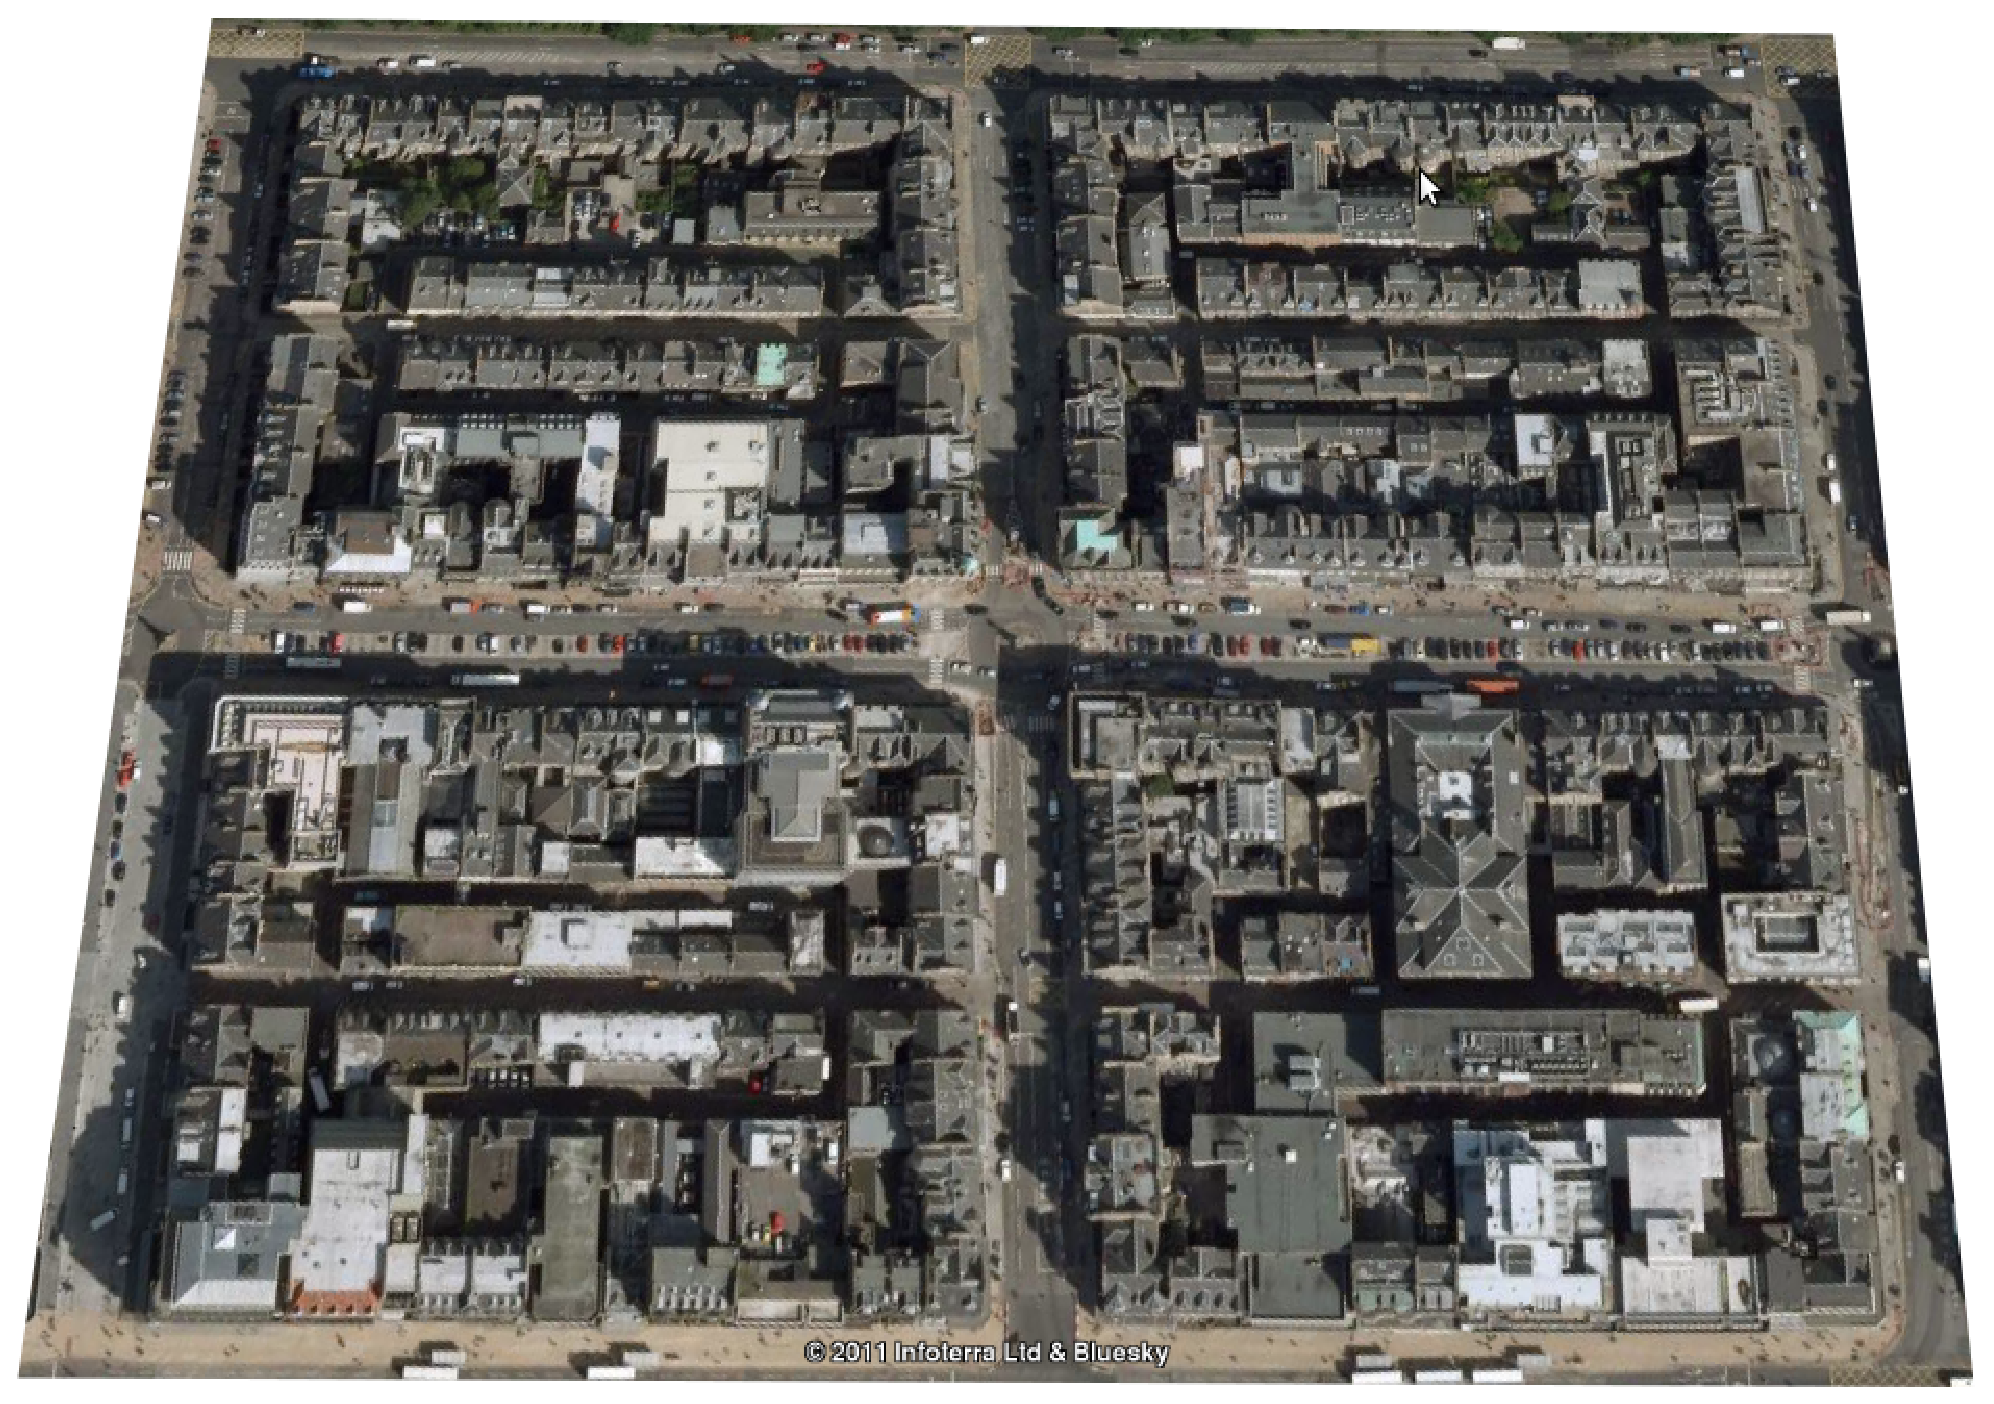
\includegraphics[width=0.40\linewidth]{images/edinburgh.eps}
\caption{Edinburgh, Princess street area}
\end{center}
\end{figure}
$$ 55^{\circ} \; 57 ^{\backprime} \; 16 ^{\backprime \backprime} \; N \; 3^{\circ} \; 11 ^{\backprime} \; 58 ^{\backprime \backprime} \; W $$ 
$$ \approx 400 \times 300 m $$
%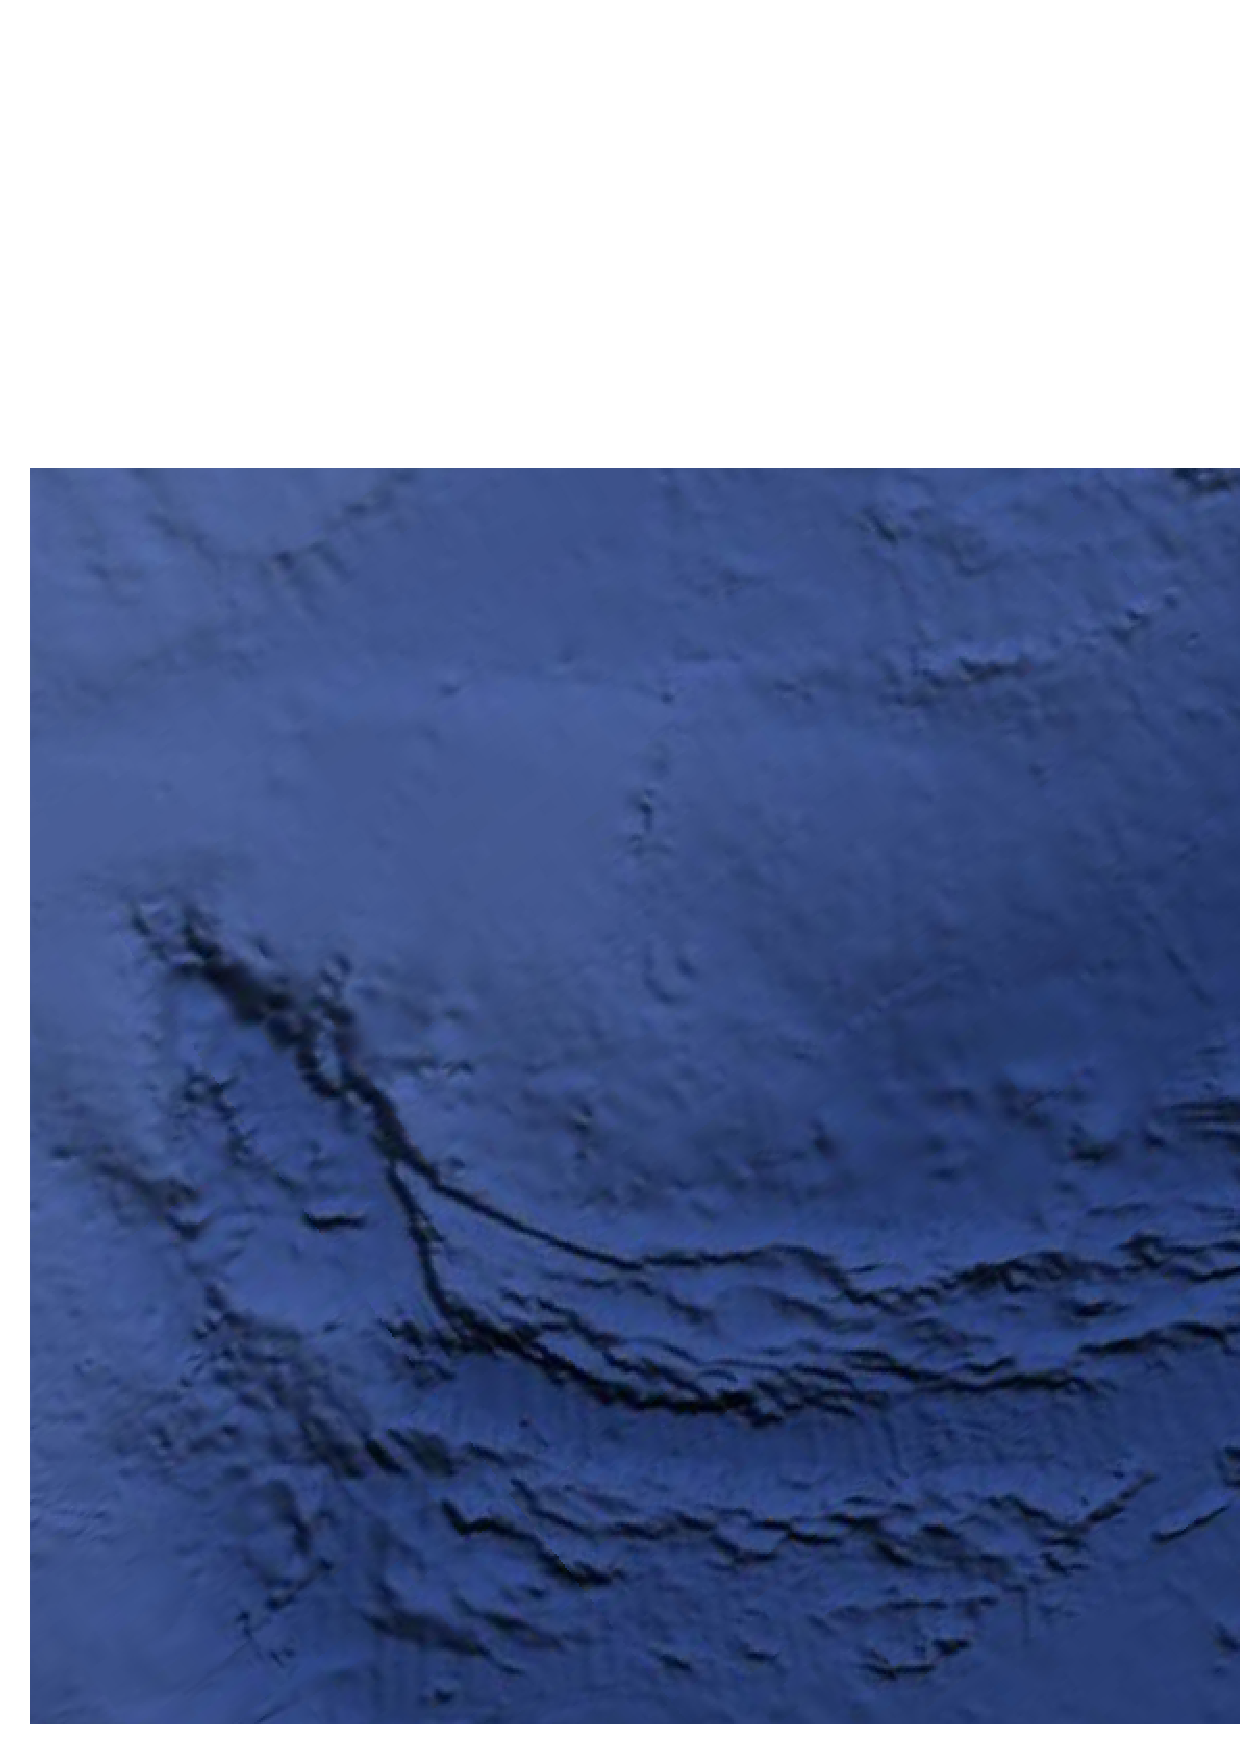
\includegraphics[height=]{images/norwegianSea.png}
1300 km away, Norwegian sea, 
$$ \approx 700 \times 300 km $$
\end{block}
\end{frame}
%%%%
\begin{frame}
			\frametitle{Sensors Description}

Brief description of navigation sensors.

\end{frame}
%%%%%
%\begin{frame}
%\frametitle{Kalman Filter Theorem}
%\begin{theorem}
%Prediction - Correction idea.
%Probabilities.
%Nonlinearity.
%EKF, UKF.
%\end{theorem}
%\end{frame}
%%%%%
%\begin{frame}
%\frametitle{Kalman fusion strategy}
%Describe the algorithm used.
%\end{frame}
%%%%%
%\begin{frame}
%\frametitle{Localisation algorithm}
%Describe the algorithm used and the ones that were tested.
%\end{frame}
%%%%%
%\begin{frame}
%\frametitle{Graphical results}
%2d plots of some missions.
%Experimental results in real environment presented.
%\end{frame}
%%%%%
%\begin{frame}
%\frametitle{Accuracy of the system}
%Interpretation of the results.
%\end{frame}
%%%%%
%\begin{frame}[fragile] % Notice the [fragile] option beside \begin{frame} %
%\frametitle{Verbatim}
%\begin{example}[Putting Verbatim]
%\begin{verbatim}
%\begin{frame}
%\frametitle{Outline}
%\begin{block}
%{Why Beamer?}
%Does anybody need an introduction to Beamer?
%I don't think so.
%\end{block}
%\end{frame}\end{verbatim} % Extra carriage return causes problem wit verbatim %
%\end{example}
%\end{frame}

\begin{frame}[fragile]  % notice the fragile ooption, since the body
			% contains a verbatim command
Example of the \verb|\cite| command to give a reference is below:

With an example of citation, \cite{key1}, we may proceed to the Bibliograhy section.
\end{frame}

\begin{frame}
\frametitle{References}
\footnotesize{
\begin{thebibliography}{99}
 \bibitem[Label1, 2010]{key1} Author's name (1987)
 \newblock Title of the paper.
 \newblock \emph{Journal Name} 55(4), 765 -- 799.
\end{thebibliography}
}
\end{frame}

\begin{frame}
\centerline{The End}
\end{frame}


% End of slides
\end{document} 